\documentclass{article}
\usepackage{listings}
\usepackage{graphicx}
\usepackage{amsmath}

\newcommand{\PRISM}{\textsc{prism}}

\date{\today}
\author{Marco Tinacci}
\title{Experiments}

\begin{document}
\maketitle
\section*{Robot arena} % (fold)
\label{sec:robot_arena}

With this example we want to give an idea of how to translate a standard fully observable model in \PRISM{}~\cite{KwiatkowskaNP11} to a partially observable one, introducing information about the observation function.

\subsection*{Robot module} % (fold)
\label{sub:robot_module}

The module define in Listing~\ref{lst:robot} describe a deterministic robot that can move in the four directions or stand still. \texttt{init} and \texttt{actions} sections describe respectively states and actions of the robot. We introduce an \texttt{observations} section that describe how sensors react to the environment.

\begin{lstlisting}[caption=Robot module, label=lst:robot, captionpos=b, frame=single]
module robot
	// init
	x0 : [0..D-1] init ix0;
	y0 : [0..D-1] init iy0;

	// observations
	[obs_n] (!see_h & see_n & ...) -> true;
	...
	[obs_ne] (!see_h & see_n & see_e & ...) -> true;
	...

	// actions
	[act_n]	true 
		-> (x0'=max(x0-1,0));
	...
endmodule
\end{lstlisting}
% subsection robot_module (end)

\subsection*{Random robot module} % (fold)
\label{sub:random_robot_module}

The module defined in Listing~\ref{lst:random_robot} define an environmental element that is a robot that follows a random walk behavior. This module does not require any modification with respect to the fully observable model. The module define in To replicate the random robot we use the Listing~\ref{lst:replica}, in this case we consider just two random robots but the replica module can be used any number of times.

\begin{lstlisting}[caption=Random robot module, label=lst:random_robot, captionpos=b, frame=single]
module RR1
	x1 : [0..D-1] init ix1;
	y1 : [0..D-1] init iy1;

	[s1]	true -> 
		1/5 : (x1'=max(x1-1,0)) +
		1/5 : (y1'=min(y1+1,D-1)) +
		1/5 : (y1'=max(y1-1,0)) +
		1/5 : (x1'=min(x1+1,D-1)) +
		1/5 : true;
endmodule
\end{lstlisting}

\begin{lstlisting}[caption=Random robot replica, label=lst:replica, captionpos=b, frame=single]
module RR2 = RR1 
	[ x1=x2, y1=y2, s1=s2, ix1=ix2, iy1=iy2 ] 
endmodule
\end{lstlisting}
% subsection random_robot_module (end)

\subsection*{Synchronization module} % (fold)
\label{sub:synchronization_module}

To implement the desired synchronization behavior we define a module dedicated to communication and timing between the main agent and the environment (Listing~\ref{lst:synch}), in this case the robot and two other random robots.

From the code we can see that this module force an iterating sequence of actions composed in the following way:
\begin{enumerate}
	\item robot observation
	\item robot action
	\item first random robot action
	\item second random robot action
\end{enumerate}
The scheme can be easily generalized to an arbitrary number of environmental elements.

\begin{lstlisting}[caption=Synchronization module, label=lst:synch, captionpos=b, frame=single]
module Synchronizer

	// turns: robot, RR1, RR2
	turn : [0..2] init 0; 
	obs: bool init true;
	
	// [<observation set>]
	[obs_n]	(turn=0 & obs=true) 
		-> (obs'=false);
	...
	[obs_ne]	(turn=0 & obs=true) 
		-> (obs'=false);
	...

	// [<action set>]
	[act_n]	(turn=0 & obs=false) 
		-> (turn'=1) & (obs'=true);
	...

	// [<coordination set>]
	[s1]	turn=1 -> (turn'=2);
	[s2]	turn=2 -> (turn'=0);

endmodule	
\end{lstlisting}
% subsection synchronization_module (end)
\subsection*{Results} % (fold)
\label{sub:results}

% 
We considered the two LTL formulae:
\begin{itemize}
	\item $\varphi_{avoid}^k = G^{\leq k} \neg \text{collision}$
	\item $\varphi_{track}^k = F^{\leq k} \text{vision}$
\end{itemize}
and we analyzed the minimum probability starting from an arbitrary initial configuration. Labels \textit{collision} and \textit{vision} represent respectively states in which the main robot's position is the same as the position of another robot, and states in which the main robot can perceive the presence of another robot close to it. We also analyze a third formula that consider the reachability within $k$ steps of \textit{vision} and not \textit{collision}, but the results are identical to $\varphi_{track}$.

% raffinamento grana
Results are shown in Figures~\ref{fig:pmin_collision} and~\ref{fig:pmin_tracking} where we plot the probabilities step by step (fine grain in blue) and the probabilities filtered by the meaningful times, that is, the initial step of every synchronization sequence (coarse grain in red). This filtering has to be done to obtain the result we really want from the beginning, that is the minimum probability sequence considering the synchronization as an atomic operation.

% esperimenti incrementando il numero di robots
We tried to stress more the dimension of the generated model, defining the robot arena of different sizes ($D = 3,4,5$) and different number of robots ($N = 3,4,5$). In Figures~\ref{fig:pmin_collision_N5} and~\ref{fig:pmin_tracking_N5} we show the minimum probabilities of collision-avoidance and tracking inside an arena containing other $4$ robots.

This means that also the formulae need to consider the synchronization mechanism employed and described by Listing~\ref{lst:synch} and thus the number of environmental modules considered in the \PRISM{} model.

\begin{figure}[htbp]
	\centering
	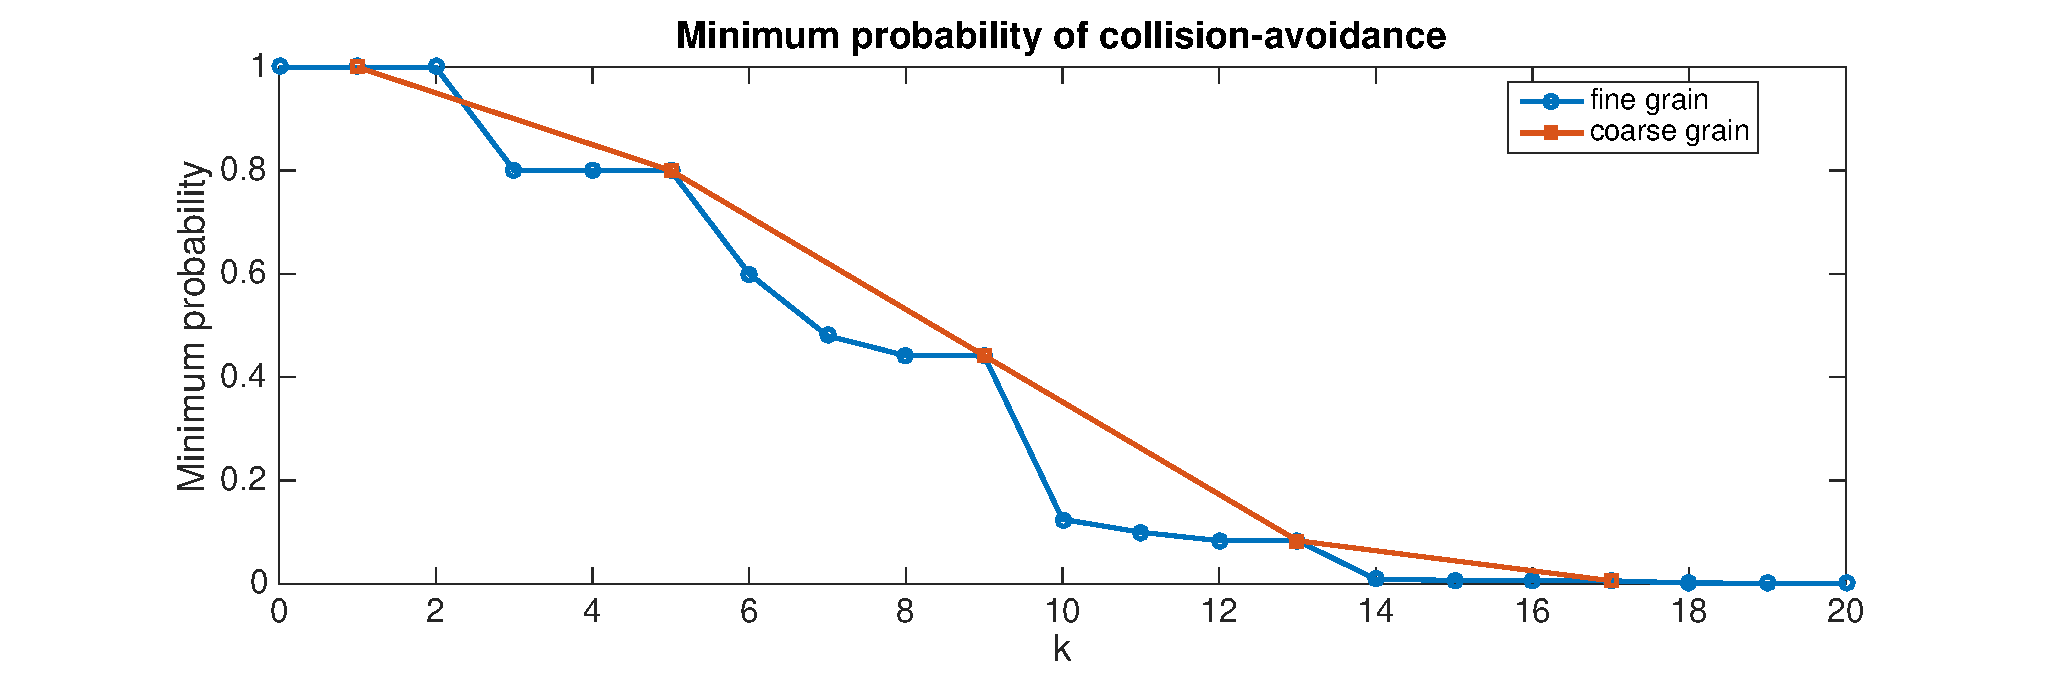
\includegraphics[width=0.95\textwidth]{figures/collision.eps}
	\caption{$\mathcal{P}_{min}\varphi_{avoid}^k$ with $3$ robots in a $3\times 3$ arena}
	\label{fig:pmin_collision}
\end{figure}
\begin{figure}[htbp]
	\centering
	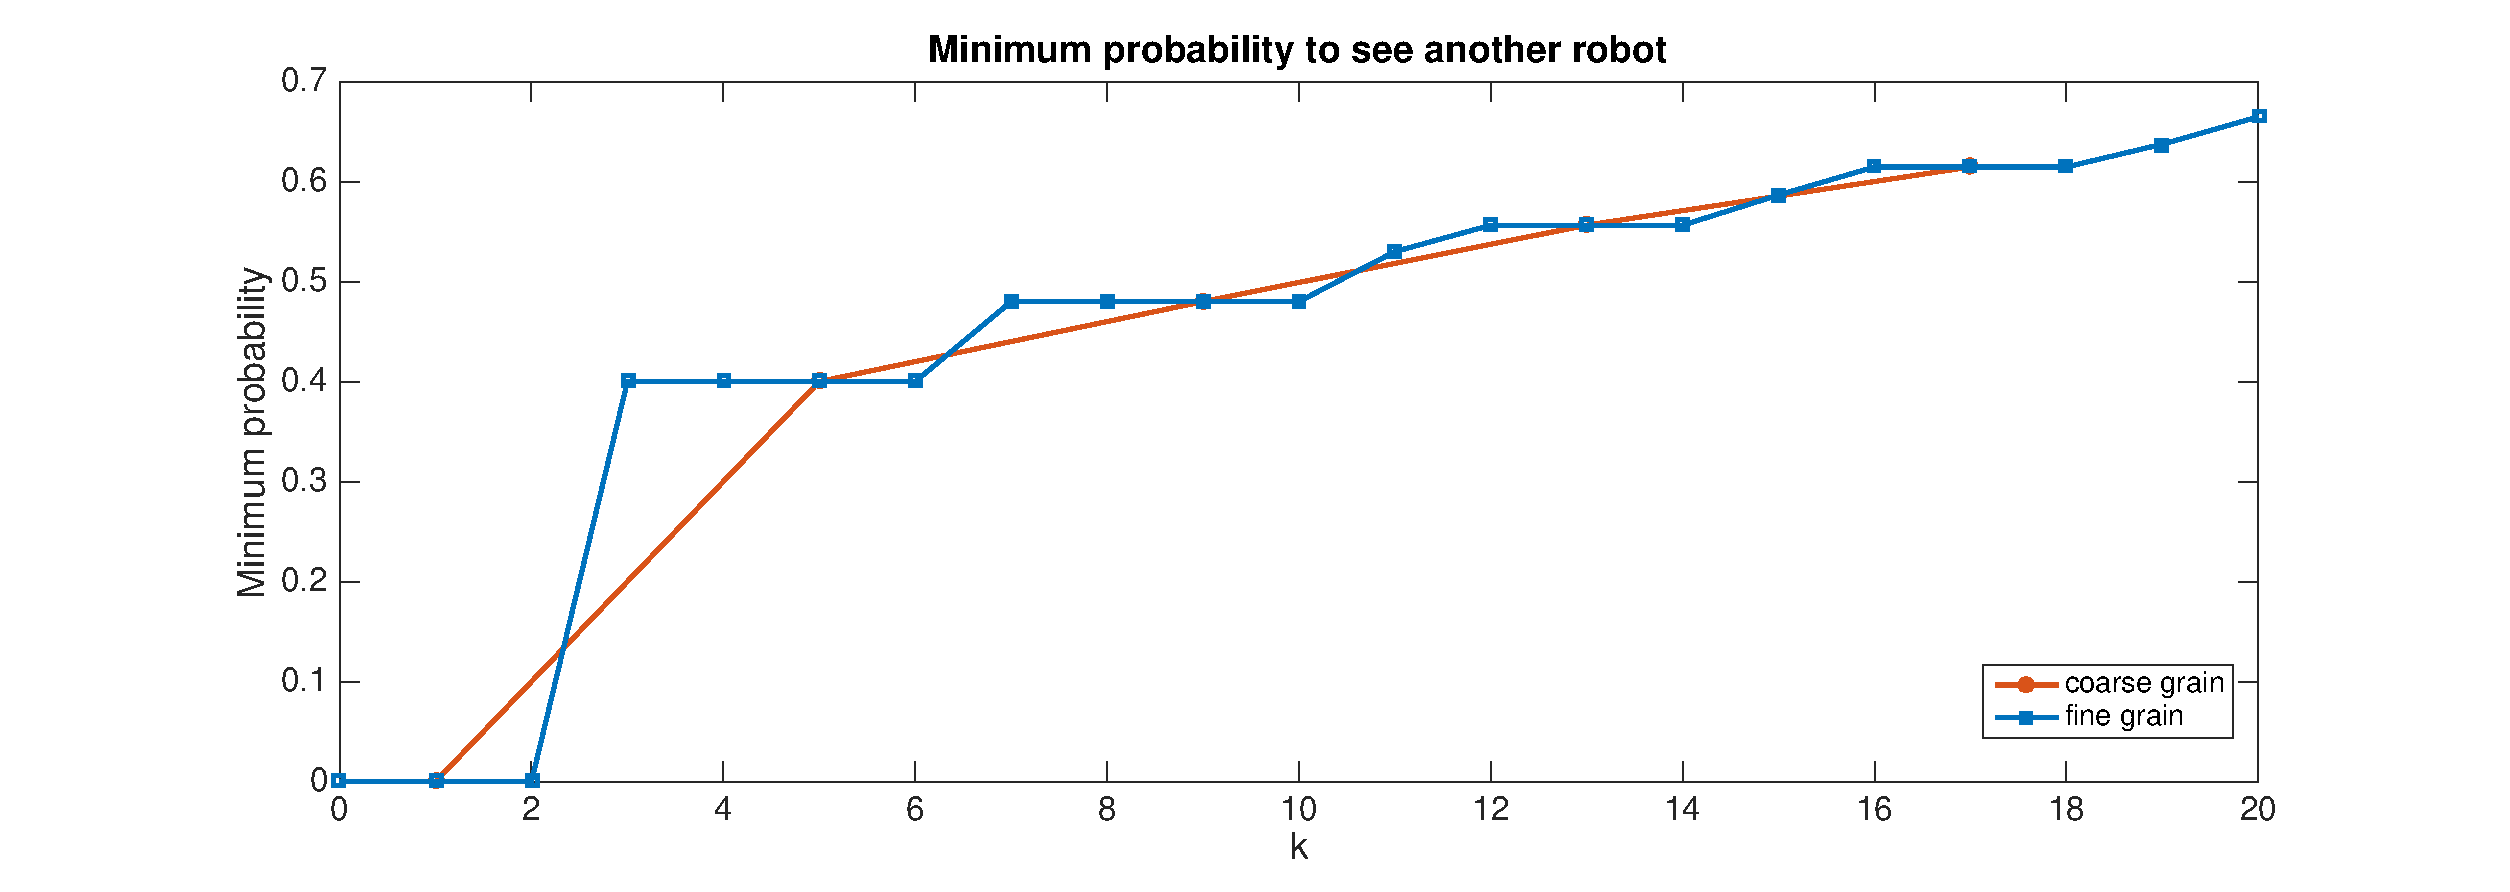
\includegraphics[width=0.95\textwidth]{figures/tracking.eps}
	\caption{$\mathcal{P}_{min}\varphi_{track}^k$ with $3$ robots in a $3\times 3$ arena}
	\label{fig:pmin_tracking}
\end{figure}
\begin{figure}[htbp]
	\centering
	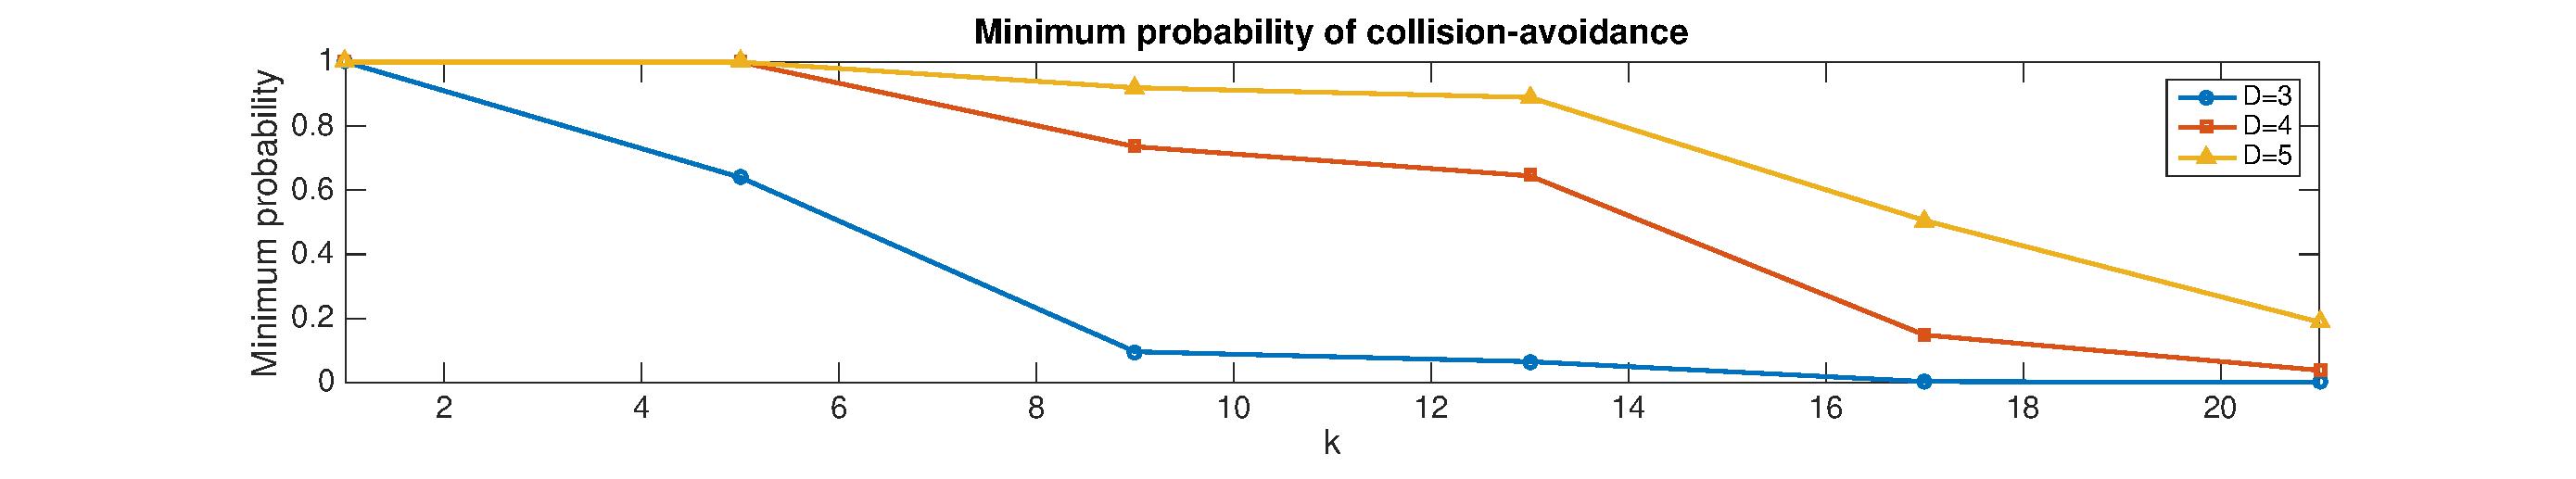
\includegraphics[width=0.95\textwidth]{figures/collisions_N5.eps}
	\caption{$\mathcal{P}_{min}\varphi_{avoid}^k$ with $5$ robots in arenas of different sizes}
	\label{fig:pmin_collision_N5}
\end{figure}
\begin{figure}[htbp]
	\centering
	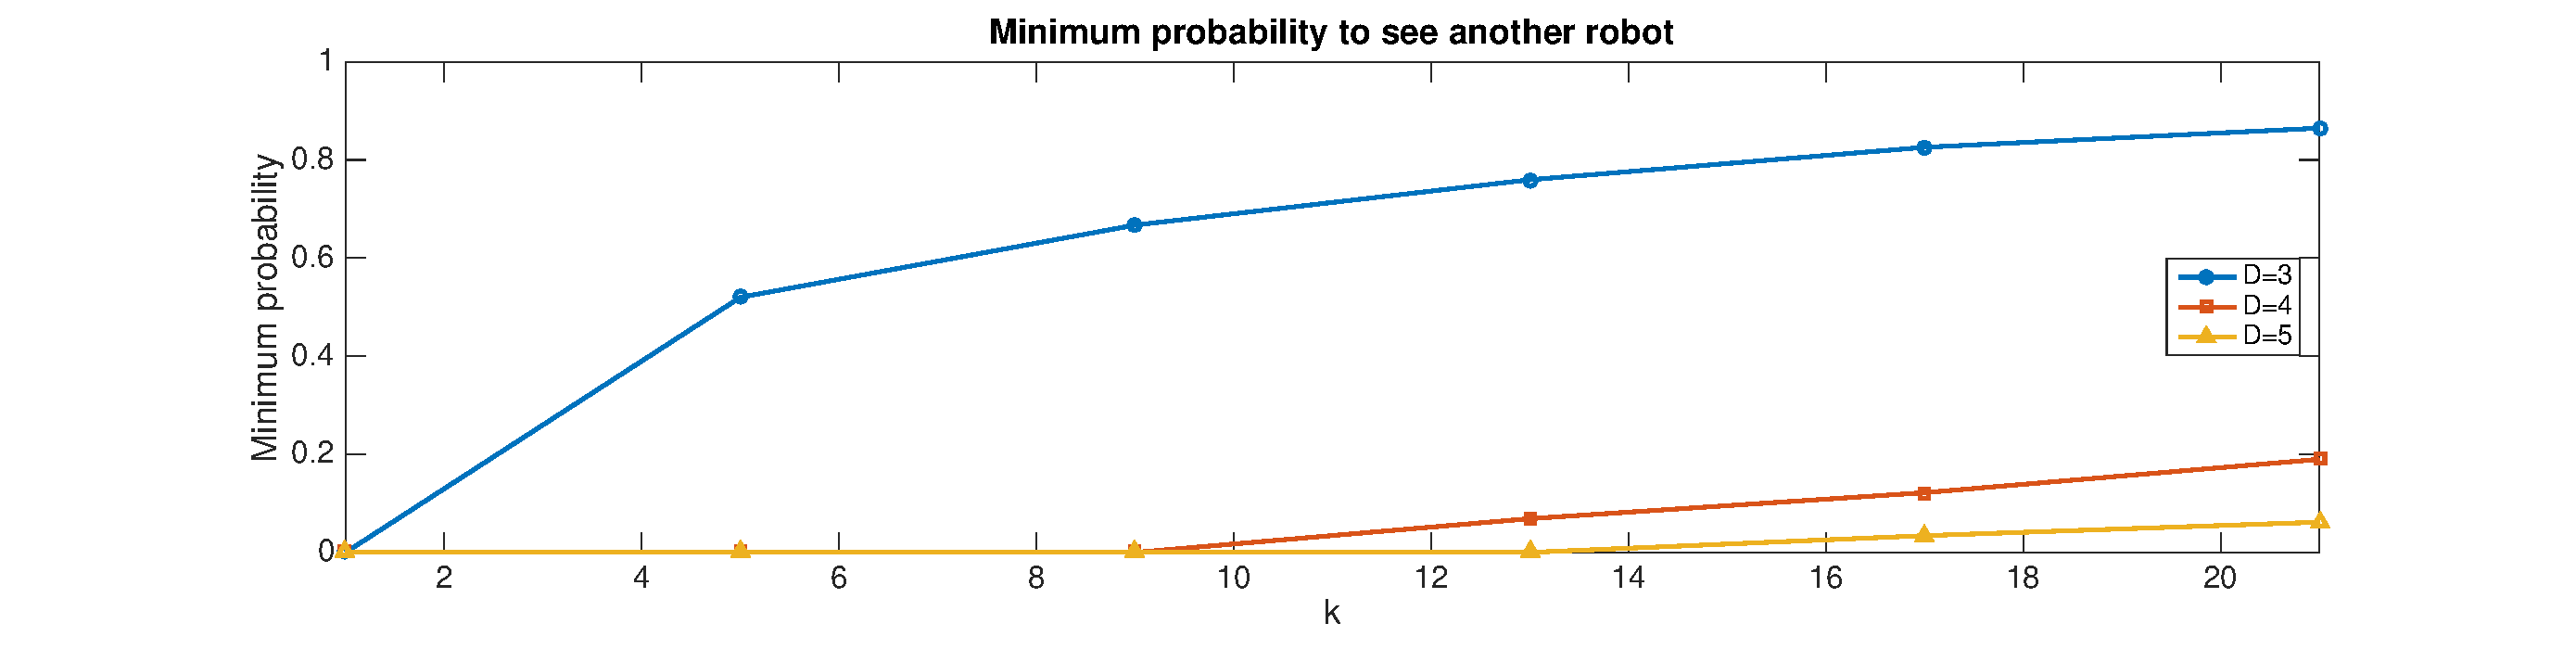
\includegraphics[width=0.95\textwidth]{figures/tracking_N5.eps}
	\caption{$\mathcal{P}_{min}\varphi_{track}^k$ with $5$ robots in arenas of different sizes}
	\label{fig:pmin_tracking_N5}
\end{figure}

% subsection results (end)
% section robot_arena (end)

\subsection*{Considerations} % (fold)
\label{sub:considerations}

Extending the fully observable \PRISM{} model into a partial observable one let us exploit its optimized engine, spareing a lot of computations with respect to the generation of the composed model. Indeed it is also possible to increase the number of robots to $5$ and to obtain .

% subsection considerations (end)

\bibliographystyle{plain}
\bibliography{biblio}
\end{document}